\chapter{Results}

This chapter presents the results of the improvement of the calibration process and object detection, tracking and labelling system.

\section{Camera Calibration}

Figure \ref{fig:gui} presents the multisensor calibration \gls{gui}. One of the SICK LMS151 \gls{lidar}s was used as point of reference for the purpose of demonstration and to have a comparator point to the camera.

\begin{figure}[htp]
	
	\centering
	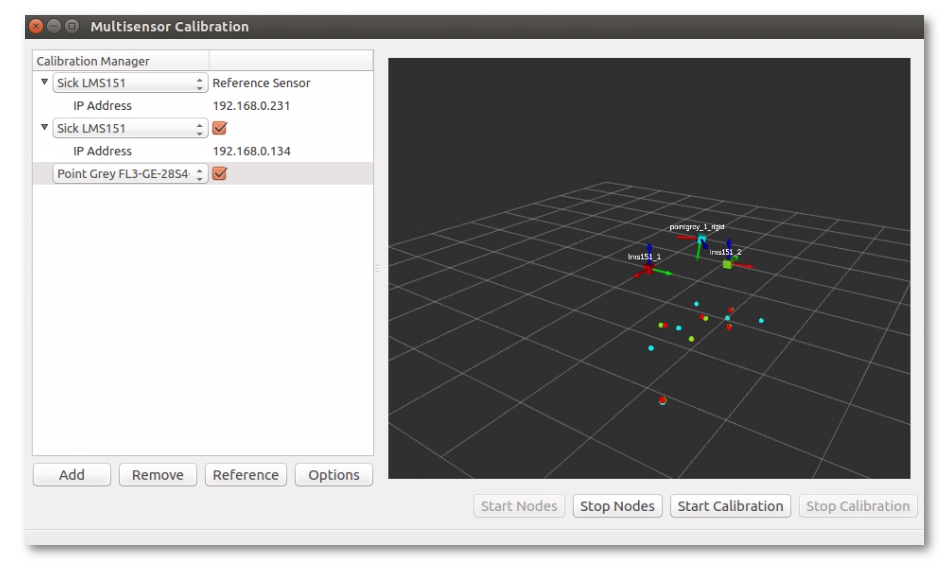
\includegraphics[width=0.9\textwidth]{capresults/imgs/gui.png}
	
	\caption{Calibration GUI with calibration result}
	\label{fig:gui}
	
\end{figure}

During the calibration procedure, the ball rolls in front of the camera and sensors. The range based sensors and the camera obtain a pointcloud of centroids of the ball during this activity. In the end, the transforms for each sensor are calculated, aligning the pointclouds of the several devices with each other. 

\begin{figure}
	\begin{center}
		\begin{lstlisting}[label={lst:calib_result}, caption={Calibration output file.},language=c++]
		-0.0563334  -0.998402 0.00440481   -1.07636
		0.997797 -0.0561436  0.0353294    1.08224
		-0.0350256 0.00638533   0.999366  0.0617893
		0          0          0          1	\end{lstlisting}
	\end{center}
\end{figure}

In listing \ref{lst:calib_result} an example output file of the calibration can be observed. The file contains a 4x4 matrix that indicates the transforms for the given sensor. Each sensor in the calibration will output its own file containing its transformation matrix relatively to the reference sensor. The reference sensor does not create a transform because it is assumed that this sensor is in the origin, unrotated. 

\section{Detection, Tracking and Labelling}

This section will present the detection, tracking and labelling results with two rosbags recorded and used for the testing of the detection, tracking and labelling algorithms. Two rosbags were recorded:

\begin{itemize}
	\item The first rosbag was recorded while leaving Departamento de Engenharia Mec\^anica at Universidade de Aveiro. The car travelled around the campus and visited the Alboi neighbourhood.
	\begin{itemize}
	\item In this bag there are cars, vans, cyclists and pedestrians. It is a bag where the car also runs into slopes. It is a rosbag with more detail which was used later in the project.
	\end{itemize} 
	\item The second rosbag starts at Alboi where the first rosbag stopped. The car follows a path into the A25 highway until the first exit.
	\begin{itemize}
	\item There are mostly cars in this one and it was a good rosbag to start with some tests in tracking objects.
	\end{itemize} 
\end{itemize} 


Each rosbag produced a dataset where the objects found were registered. Looking into the datasets can show how the algorithm behaves.

\subsection{Dataset 1 - Highway / A25}

The first dataset was produced from the highway rosbag. The rosbag duration is 3:37s (217s), has a size of 8.6 GB and includes 62352 messages.

The labelling was done using semi-automatic methods using sensor fusion and also manually by pointing and clicking on an object when the sensors don't find it. The semi-automatic methods suggest the user an object of interest and asks for a label from the user.

\begin{table}[]
	\centering
	\caption{Highway dataset annotation metrics}
	\label{tab: highwaymetrics}
	\begin{tabular}{c|c}
		\textbf{Metric}      & \textbf{Count} \\ \hline
		\textbf{\begin{tabular}[c]{@{}c@{}}Right\\ Suggestions\end{tabular}}            & 12             \\ \hline
		\textbf{\begin{tabular}[c]{@{}c@{}}Wrong\\ Suggestions\end{tabular}}            & 6              \\ \hline
		\textbf{\begin{tabular}[c]{@{}c@{}}Manual\\ Entries Saved\end{tabular}}         & 1              \\ \hline
		\textbf{\begin{tabular}[c]{@{}c@{}}Manual Entries\\ Discarded\end{tabular}}     & 0              \\ \hline
		\textbf{\begin{tabular}[c]{@{}c@{}}Maximum Objects\\ in One Frame\end{tabular}} & 1             
	\end{tabular}
\end{table}

Several objects were found in this sequence. The discarded objects or the objects wrongly suggested by the semi-automatic system are still saved but labelled as \texttt{DontCare}. Other labels used are \texttt{car}, \texttt{van}, \texttt{people}, \texttt{bicycle}, \texttt{sign} (street signs) and \texttt{misc} (miscellaneous objects in the streets like dumpsters, bushes and trees). The amount of objects found in this rosbag is listed in table \ref{tab: highwaystats}.

\begin{table}[]
	\centering
	\caption{Highway dataset object amounts}
	\label{tab: highwaystats}
	\begin{tabular}{c|c|c|c|c|c|c|c|c}
		\textbf{Label} & \texttt{car} & \texttt{van} & \texttt{people} & \texttt{bicycle} & \texttt{sign} & \texttt{misc} & \texttt{DontCare} & \textbf{total} \\ \hline
		\textbf{Count} & 7            & 1            & 0               & 0                & 4             & 1             & 6                 & 19            
		 
	\end{tabular}
\end{table}

As this sequence presents few objects at a time, most semi-automatic suggestions were accepted. The semi-automatic system works better in areas with reduced movement so the readings of the sensors are more accurate.

\subsection{Dataset 2 - Aveiro City Urban Area}

The second dataset was generated from the rosbag at an urban area in Aveiro city. The rosbag duration is 7:06s (456s), has a size of 18.0 GB and includes 135379 messages. 

The labelling in this rosbag was done using the semi-automatic methods and the manual methods separately. The reason for this is to compare the behavior of the semi-automatic suggestions and the manual method in a different environment.

\subsubsection{Dataset 2.1 - Semi-Automatic Method}

The dataset produced with the semi-automatic method the labelling metric listed in table \ref{tab: urban1metrics}.

\begin{table}[]
	\centering
	\caption{Urban area dataset with semi-automatic methods annotation metrics}
	\label{tab: urban1metrics}
	\begin{tabular}{c|c}
		\textbf{Metric}              & \textbf{Count} \\ \hline
		Right Suggestions            & 36                      \\ \hline
		Wrong Suggestions            & 74                      \\ \hline
		Maximum Objects In One Frame & 1                      
	\end{tabular}
\end{table}

The Urban area is a zone with high-traffic and because there are more objects (sidewalks, road boundaries, walls, etc...), the semi-automatic method is more likely to mistake an object of interest with something with no significance in the dataset scope. 

The metrics show that nearly 2 out of 3 suggestions are something that has no interest for the dataset. In table \ref{tab: urban1stats} the amount of objects found is presented.

\begin{table}[]
	\centering
	\caption{Urban area dataset  with semi-automatic methods object amounts}
	\label{tab: urban1stats}
	\begin{tabular}{c|c|c|c|c|c|c|c|c}
		\textbf{Label} & \texttt{car} & \texttt{van} & \texttt{people} & \texttt{bicycle} & \texttt{sign} & \texttt{misc} & \texttt{DontCare} & \textbf{total} \\ \hline
		Count          & 29           & 2            & 4               & 0                & 1             & 0             & 74                & 110           
	\end{tabular}
\end{table}


\subsubsection{Dataset 2.2 - Manual Method}

To test the manual method, one must click on the object and control the rosbag (pause it, go back and forward, etc...) to obtain maximum precision on the detection and tracking. 

\begin{table}[]
	\centering
	\caption{Urban area dataset with manual methods annotation metrics}
	\label{tab: urban2metrics}
	\begin{tabular}{c|c}
		\textbf{Metric}              & \textbf{Count} \\ \hline
		Entries Saved           & 89                      \\ \hline
		Entries Discarded            & 31                      \\ \hline
		Maximum Objects In One Frame & 4                 
	\end{tabular}
\end{table}

In table \ref{tab: urban2metrics} some annotation metrics are shown. Despite the high traffic zone, the metrics in the manual methods show that nearly 3 out of 4 clicks result in a good detection and tracking of the object. 

Because the annotation was done manually, it is possible to enter more than one object at the same time whereas in the semi-automatic that is not possible because when the sensors suggest an object in sight, the algorithm always outputs the object that is closer to the vehicle. In table \ref{tab: urban2stats} it is possible to see the amount of each object in this dataset.

\begin{table}[]
	\centering
	\caption{Urban area dataset with manual methods object amounts}
	\label{tab: urban2stats}
	\begin{tabular}{c|c|c|c|c|c|c|c|c}
		\textbf{Label} & \texttt{car} & \texttt{van} & \texttt{people} & \texttt{bicycle} & \texttt{sign} & \texttt{misc} & \texttt{DontCare} & \textbf{total} \\ \hline
		Count          & 63           & 10            & 10               & 2                & 1             & 3             & 31                & 120           
	\end{tabular}
\end{table}

Analyzing table \ref{tab: urban2stats} it is possible to conclude that with manual methods one can freely enter with more detail the detected objects. In comparison to the semi-automatic methods, with the manual strategy it is easier to enter objects like people and bicycles as it seems to be difficult to cluster such small objects in the given sensor data.











